% --------------------------------------------------------------------------------

\begin{exercise}

Berechnen Sie die greensche Funktion $G(x, y, \xi, \eta)$ für $\Delta$ auf der Viertelebene

\begin{align*}
  \Omega
  =
  \Bbraces{(x, y) \in \R^2: x > 0, y > 0}
\end{align*}

mit Hilfe der Spiegelungsmethode.
  Stellen Sie mit dieser greenschen Funktion die Lösung des Dirichlet-Problems

\begin{align*}
  \Delta u = 0 ~\text{in}~ \Omega,
  \quad
  u(x, 0) = f(x) ~\text{für}~ x > 0,
  \quad
  u(0, y) = g(y) ~\text{für}~ y > 0
\end{align*}

dar, wobei $f$ und $g$ stetig und beschränkt auf $(0, \infty)$ sind. Ist diese Lösung eindeutig?

\end{exercise}

% --------------------------------------------------------------------------------

\begin{solution}

\phantom{}

\begin{figure}[h!]
  \centering
  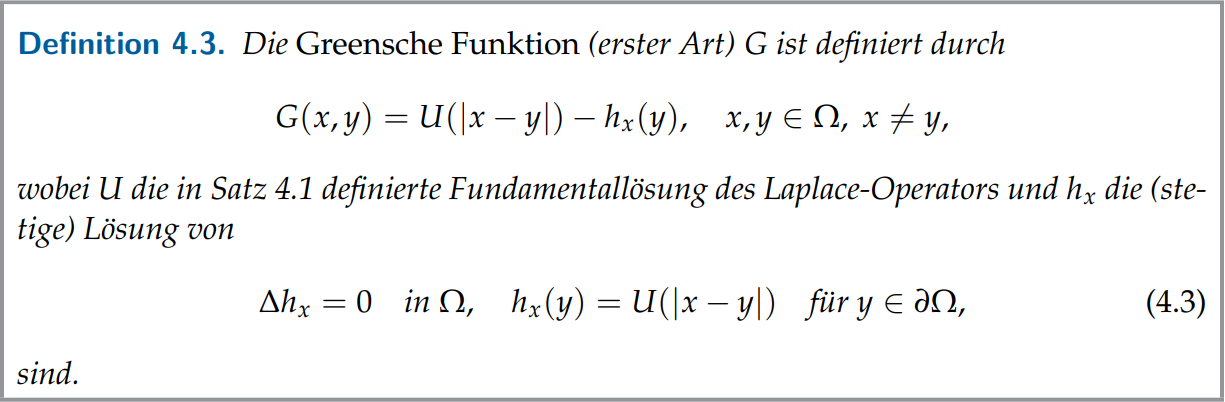
\includegraphics
  [width = 0.75 \textwidth]
  {Definition 4-3.png}
\end{figure}

%\includegraphicsboxed{(4-4).png}

Wir verwenden die Fundamentallösung im $\R^2$,

\begin{align*}
  U(x, y)
  =
  \frac{1}{2 \pi}
  \ln \sqrt{x^2 + y^2},
  \quad
  (x, y) \in \R^2,
  (x, y) \neq (0, 0).
\end{align*}

Die Spiegelungsmethode liefert nach richtiger Anwendung beide Teile von (4.4).

\begin{enumerate}

  \item Nachdem wir, durch addieren von gespiegelten Fundamentallösungen, nur Pole außerhalb von $\Omega$ einführen, und uns auf $\Omega$ am Ende beschränken, ist der erste Teil automatisch gegeben.

  \item Wir wollen im zweiten Teil, dass die Greensche Funktion mit $(\xi, \eta) \in \partial \Omega$ verschwindet.
  Schematisch lässt sich das mit Matrizen ausdrücken.
  Der Text unter den Matrizen soll die Spiegelung beschreiben.
  Die Summe der Matrizen soll (auf dem Rand) $0$ werden.

  \begin{align*}
    \underbrace
    {
      \begin{pmatrix}
          & N &   \\
        W &   & O \\
          & S &
      \end{pmatrix}
    }_{
      \text{keine}
    }
    -
    \underbrace
    {
      \begin{pmatrix}
          & S &   \\
        W &   & O \\
          & N &
      \end{pmatrix}
    }_{
      x ~\text{Achse}
    }
    -
    \underbrace
    {
      \begin{pmatrix}
          & N &   \\
        O &   & W \\
          & S &
      \end{pmatrix}
    }_{
      y ~\text{Achse}
    }
    +
    \underbrace
    {
      \begin{pmatrix}
          & S &   \\
        O &   & W \\
          & N &
      \end{pmatrix}
    }_{
      x \& y ~\text{Achse}
    }
    =
    0
  \end{align*}

\end{enumerate}

Insgesamt erhalten wir durch die Spiegelungsmethode folgenden Kandidaten für die Greensche Funktion.

\begin{align*}
  G(x, y, \xi, \eta)
  & =
  U \pbraces
  {
    \vbraces
    {
      \begin{pmatrix}
        x \\ y
      \end{pmatrix}
      -
      \begin{pmatrix}
        \xi \\ \eta
      \end{pmatrix}
    }
  }
  -
  h_{(x, y)}
  \begin{pmatrix}
    \xi \\ \eta
  \end{pmatrix} \\
  & =
  U \pbraces
  {
    \vbraces
    {
      \begin{pmatrix}
        x \\ y
      \end{pmatrix}
      -
      \begin{pmatrix}
        \xi \\ \eta
      \end{pmatrix}
    }
  }
  -
  U \pbraces
  {
    \vbraces
    {
      \begin{pmatrix}
        x \\ y
      \end{pmatrix}
      -
      \begin{pmatrix}
        -\xi \\ \eta
      \end{pmatrix}
    }
  }
  -
  U \pbraces
  {
    \vbraces
    {
      \begin{pmatrix}
        x \\ y
      \end{pmatrix}
      -
      \begin{pmatrix}
        \xi \\ -\eta
      \end{pmatrix}
    }
  }
  +
  U \pbraces
  {
    \vbraces
    {
      \begin{pmatrix}
        x \\ y
      \end{pmatrix}
      -
      \begin{pmatrix}
        -\xi \\ -\eta
      \end{pmatrix}
    }
  } \\
  & =
  \frac{1}{2 \pi}
  \Big (
    \ln \sqrt{(x + \xi)^2 + (y + \eta)^2}
    +
    \ln \sqrt{(x - \xi)^2 + (y + \eta)^2} \\
    & \qquad +
    \ln \sqrt{(x + \xi)^2 + (y + \eta)^2}
    +
    \ln \sqrt{(x + \xi)^2 + (y + \eta)^2}
  \Big ) \\
  & =
  \frac{1}{4 \pi}
  \Big (
    \ln ((x + \xi)^2 + (y + \eta)^2)
    +
    \ln ((x - \xi)^2 + (y + \eta)^2) \\
    & \qquad +
    \ln ((x + \xi)^2 + (y + \eta)^2)
    +
    \ln ((x + \xi)^2 + (y + \eta)^2)
    \Big )
  \end{align*}

  \begin{figure}[h!]
    \centering
    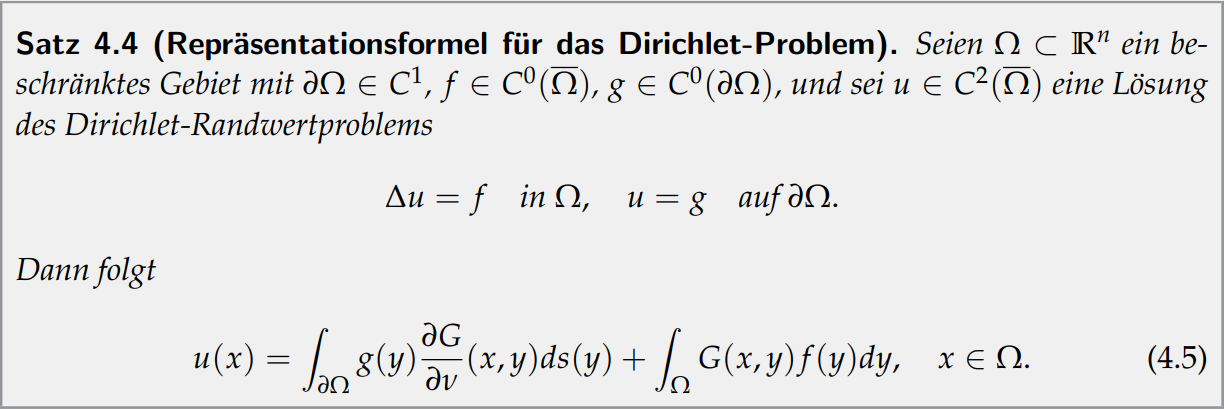
\includegraphics
    [width = 0.75 \textwidth]
    {Satz 4-4 (Repraesentationsformel fuer das Dirichlet-Problem.png}
  \end{figure}

  Wir wollen die Repräsentationsformel für das Dirichlet-Problem benutzen.
  Unsere Rand-Funktionen können wir zu einer zusammenfassen.

  \begin{align*}
    h:
    \partial \Omega \to \C:
    (x, y)
    \mapsto
    \begin{cases}
      u(0, y) = g(y), & x = 0, \\
      u(x, 0) = f(x), & y = 0
    \end{cases}
  \end{align*}

  Weil unser Dirichlet-Problem homogen ist, fällt das zweite Integral von (4.5) weg.
  Wir erhalten somit folgende Repräsentation von $u$.

  \begin{align*}
    u(x, y)
    =
    \Int[\partial \Omega]
    {
      h(\xi, \eta)
      \pderivative[][G]{\nu}
      (x, y, \xi, \eta)
    }{
      s(\xi, \eta)
    }
    =
    -\Int[0][\infty]
    {
      \underbrace{h(0, \eta)}_{g(\eta)}
      \underbrace
      {
        \pderivative[][G]{\xi}
        (x, y, 0, \eta)
      }_{
        =: K_\xi(x, y, \eta)
      }
    }{\eta}
    -\Int[0][\infty]
    {
      \underbrace{h(\xi, 0)}_{f(\xi)}
      \underbrace
      {
        \pderivative[][G]{\eta}
        (x, y, \xi, 0)
      }_{
        =: K_\eta(x, y, \xi)
      }
    }{\xi}
  \end{align*}

  Wir berechnen die (eigentlich negativen) Kerne explizit.

  \begin{comment}

  \begin{align*}
    K_\xi(x, y, \eta)
    =
    \frac
    {
      x
      (
        (\eta - y)^2
        -
        (\eta + y)^2
      )
    }{
      \pi
      (x^2 + (\eta - y)^2)
      (x^2 + (\eta + y)^2)
    },
    \quad
    K_\eta(x, y, \xi)
    =
    \frac
    {
      y
      (
        (x - \xi)^2
        -
        (x + \xi)^2
      )
    }{
      \pi
      (y^2 + (x - \xi)^2)
      (x^2 + (x + \xi)^2)
    }
  \end{align*}

  \end{comment}

  \begin{align*}
    K_\xi(x, y, \eta)
    =
    \frac{1}{\pi}
    \pbraces
    {
      \frac{x}{x^2 + (y + \eta)^2}
      +
      \frac{x}{x^2 + (y - \eta)^2}
    },
    \quad
    K_\eta(x, y, \xi)
    =
    \frac{1}{\pi}
    =
    \frac{1}{\pi}
    \pbraces
    {
      \frac{y}{y^2 + (x + \xi)^2}
      +
      \frac{y}{y^2 + (x - \xi)^2}
    }
  \end{align*}

  Wir berechnen deren Integrale.

  \begin{align*}
    I_\eta
    & :=
    \Int[0][\infty]{K_\xi(x, y, \eta)}{\eta}
    =
    \frac{1}{\pi}
    \pbraces
    {
      \arctan_2
      \begin{pmatrix}
        x \\ y
      \end{pmatrix}
      -
      \arctan_2
      \begin{pmatrix}
        x \\ -y
      \end{pmatrix}
    }
    \stackrel{x > 0}{=}
    \frac{1}{\pi}
    \pbraces
    {
      \arctan \frac{y}{x}
      -
      \arctan -\frac{y}{x}
    }
    =
    \frac{2}{\pi} \arctan \frac{y}{x} \\
    I_\xi
    & :=
    \Int[0][\infty]{K_\eta(x, y, \xi)}{\xi}
    =
    \frac{1}{\pi}
    \pbraces
    {
      \arctan_2
      \begin{pmatrix}
        y \\ x
      \end{pmatrix}
      -
      \arctan_2
      \begin{pmatrix}
        y \\ -x
      \end{pmatrix}
    }
    \stackrel{y > 0}{=}
    \frac{1}{\pi}
    \pbraces
    {
      \arctan \frac{x}{x}
      -
      \arctan -\frac{x}{y}
    }
    =
    \frac{2}{\pi} \arctan \frac{x}{y} \\
  \end{align*}

  Um zu sehen, dass die Summe der Integrale konstant gleich $1$ ist, bemerken wir, dass dies für $x := y := 1$ gilt, und die Ableitungen nach $x$ und $y$ verschwinden.

  \begin{align*}
    \implies
    I
    :=
    I_\xi + I_\eta
    =
    \frac{2}{\pi}
    \pbraces
    {
      \arctan \frac{x}{y}
      +
      \arctan \frac{y}{x}
    }
    =
    1
  \end{align*}

  Der erste Teil von (4.4) funktioniert analog zu Beweis von Satz 4.5.
  Der zweite Teil nicht ganz ...

  \begin{align*}
    u(x, y)
    \begin{cases}
      \xrightarrow[y \to 0]{x \to x_0} f(x_0), \\
      \xrightarrow[x \to 0]{y \to y_0} g(y_0).
    \end{cases}
  \end{align*}

  Weil das sehr aufwändig ist, tun wir das aber nur für die $x$-Achse.

  \begin{align*}
    |u(x, y) - f(x_0)|
    & =
    \vbraces
    {
      \Int[0][\infty]
      {
        g(\eta)
        K_\xi(x, y, \eta)
      }{\eta}
      +
      \Int[0][\infty]
      {
        f(\xi)
        K_\eta(x, y, \xi)
      }{\xi}
      -
      f(x_0) \cdot I
    } \\
    & \leq
    \underbrace
    {
      \Int[0][\infty]
      {
        K_\xi(x, y, \eta)
        |g(\eta) - f(x_0)|
      }{\eta}
    }_{\cdots}
    +
    \underbrace
    {
      \Int[0][\infty]
      {
        K_\eta(x, y, \xi)
        |f(\xi) - f(x_0)|
      }{\xi}
    }_{
      \text{siehe Beweis von Satz 5.4}
    }
  \end{align*}

  Das zweite Integral wird im Beweis von Satz 4.5 abgeschätzt;
  Wir kümmern uns daher bloß um das erste.
  Dazu bemerken wir, dass $g$ und $f$ beschränkt sind.

  \begin{align*}
    \cdots \leq \sup_{\eta \in (0, \infty)}
      |g(\eta) - f(x_0)|
    \Int[0][\infty]
    {  K_\xi(x, y, \eta)}{\eta}
    = \frac{2}{\pi}\underbrace{\sup_{\eta \in (0, \infty)}
      |g(\eta) - f(x_0)|}_{< \infty}  \arctan \frac{y}{x}
      \xrightarrow{y \to 0} 0.
  \end{align*}
\end{solution}

% --------------------------------------------------------------------------------
